\documentclass{article}

\usepackage{amsmath}
\usepackage{geometry}
\usepackage{graphicx}

\author{Gideon Moore}
\date{April 3, 2024}
\title{Introductory Memo: \\ Demand Estimation Using Movie Descriptions}

\begin{document}

\maketitle

\begin{abstract}
    Traditional BLP-based demand estimation requires structured characteristic data to identify cross-elasticities. Many markets, however, feature unstructured text descriptions of products without well-structured characteristics. Using modern text-to-data tools, I hope to estimate cross-elasticities in the presence of unstructured text alone. I exploit specific characteristics of the movie industry to pilot this methodology. Uniform pricing is ubiquitous in this market; thus, we can make arguments about demand shifts from quantity changes alone. Moreover, long and inflexible production pipelines have the potential to produce plausibly-exogeneous product characteristics; this argument is supported by the presence of ``twin films,'' movies released simultaneously which are so similar they cannibalize each other's sales. 
\end{abstract}

\section{Research Question}

BLP is a workhorse for estimating cross-elasticities between products; however, the technique lives in the characteristic space. We need an ontological understanding of these products: what they are, and why each characteristic matters. The econometrician makes a judgement call about whether, e.g., car size is a factor in people's decision to purchase a car. Moreover, these characteristics need to be somehow pre-digested: without a table of car sizes, the econometrician cannot include it in the model even if it is relevant.

Many products contain text descriptions of their characteristics. This could be a Amazon listing for a product, a Yelp summary of a restaurant, or a description of a movie. These descriptions by design include the most important information consumers need about a product, as sellers attempt to attract as many consumers as possible. Thus, if we could incorporate this data into our model, it should be highly informative about the characteristics of the product. Moreover, it removes the judgement call of the economist: the characteristics included are precisely those the merchants themselves believe to be most important. 

Thus, the question is: can we use text data to estimate cross-elasticities between products as a supplement (or substitute) for structured characteristic data?

Because text-to-data techniques have evolved so rapidly, the literature is relatively primitive; existing work usually uses algorithms from the pre-LLM era (e.g., word2vec) which are anecdotally much lower quality. Modern embedding-based methods are also strongly preferable to bag-of-words approaches for short text samples, as the odds any particular bigram appears in three sentences are quite low. I have identified two working papers from the past few months which are particularly relevant. 

Compiani et al., released last October as a CESifo working paper, uses Amazon listing text and image data to estimate a combinatorial nested logit for consumer electronics. I believe this would be my closest ``substitute'' in the literature; however, I believe I improve on their results in at least two ways. My first iteration on this paper would be an improvement in the embedding method--they use a bag-of-words, a TF-IDF, a sentence encoder, and Sentence-BERT; notably, all of these embeddings predate the advent of recent LLMs. Secondly, to me the setting for this paper is notably inferior; specifically, I do not believe there is any exogeneous variation in demand. The BLP assumption clearly does not hold here--the characteristics of the Kindle Fire 7 Kids were clearly chosen keeping the characteristics of the Kindle Fire 7 in mind. Thus, the paper seems to be entirely observational. 

Michalopoulos and Rauh, published two weeks ago as an NBER working paper, is a complementary paper which also uses movie descriptions as an input for text analysis. However, rather than using this data to estimate distances between different movies, this paper compares each movie to local myths and legends to estimate the impact of cultural proximity on movie success. In many ways this can act as a template for some of my text analysis work in the movie context; however, the thrust of my paper is almost entirely unrelated. Again, this uses a 2018 sentence encoder and the Latent Dirichlet Analysis method first published in 2003--both well predating modern text analysis tools. 

A personal note: while I think this is in some ways interesting on its own, I'm not an econometrician--for me, this is basically an intermediate good. I have another project thinking about changes in field subject matter over time; e.g., studying how a 1990 computer science major fares in the 2020 market for software engineers. I'm hoping to use text data such as course descriptions and textbook content to estimate the size of these changes by field, potentially examining substitution between hiring different majors. In that sense this is very much a ``yogurt'' paper--if I can show text data works acceptably in this simple context, I'm hoping to apply it credibly in the more complex setting down the line.

\section{Institutional Setting: Movies}

I suggest piloting this methodology in the movie industry. There are two institutional details which make this a good setting (in conjunction with data availability, which I will cover in the next section). 

\subsection{The Uniform-Price Puzzle}

As is well-documented (in one of Liran's papers, among others), the movie industry exhibits a peculiar pricing standard: all movie tickets are the same price. Thus--conditional on the movie being produced--supply of the movie is perfectly elastic. This may or may not be profit maximizing, but I leave that for other papers to explore. The point is that when demand shifts, this manifests \emph{entirely} as a change in quantity. Therefore--unlike other settings where price responds endogeneously--we can reason about demand shifts from price data alone. 

\subsection{The BLP Assumption: Twin Movies}

A critical assumption of the BLP model is that product characteristics cannot be determined in strategic response to competitors. While I think this is indefensible in the majority of industries, there exists anecdotal evidence it is true in the movie industry. 

The concept of ``twin films'' is well-known enough to have its own--quite developed--Wikipedia page. The idea is that, likely as a result of market researchers reporting similar trends to separate studios independently, two studios develop movies which are remarkably similar. Examples include \emph{A Bug's Life} and \emph{Antz} both releasing in 1998, \emph{Knocked Up} and \emph{Juno} both releasing in 2007, and \emph{No Strings Attached} and \emph{Friends with Benefits} both releasing in 2011.

Generally, twin films are considered unfortunate occurances--audiences will generally see one or the other, rather than both, leading to a significant decline in demand. If firms could avoid them, then, they would; their continued existence suggests that movie studios are in some sense inflexible in the characteristics of their products, satisfying the BLP assumption

\section{Data}

The other virtue of the movie industry is the availability of data. While IMDb is the ``preferred'' movie platform, their data is quite expensive. Fortunately, there exists an community-made competitor, TMDb, with a free API. While IMDb is certainly more comprehensive, for my purposes TMDb should be sufficient (and if this project takes off, I can consider spending the cash for the IMDb data). Figure \ref{fig:star_wars} shows the page for the original \emph{Star Wars} to illustrate what is available. All of these qualities can be retrieved via the free API.

\begin{figure}[h]
    \centering
    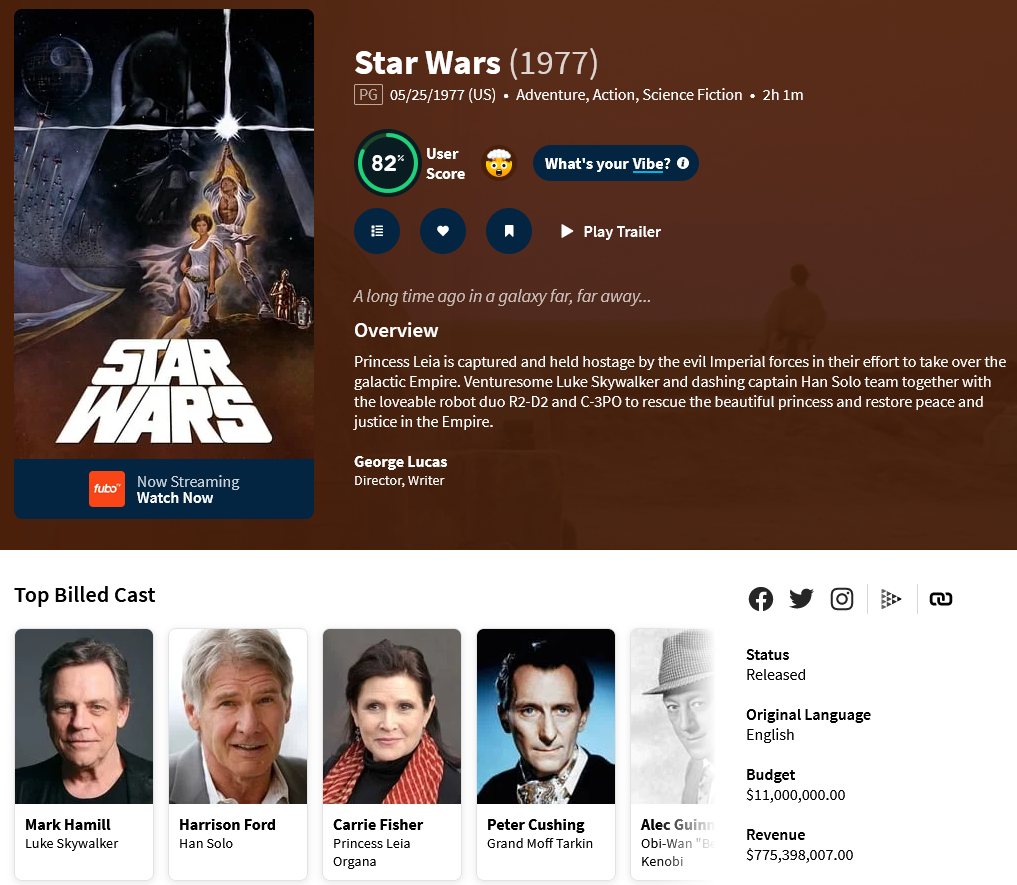
\includegraphics[width=0.8\textwidth]{star_wars_tmdb.png}
    \caption{Screenshot of the TMDb page for \emph{Star Wars}}
    \label{fig:star_wars}
\end{figure}

As far as outcome variables are concerned, I have two options as measures of ``quantity.'' The classic approach would be to use some version of box office receipts over time. Alternatively, I also considered using Google Search trends. To me, both of these seem like expressions of interest in the movie; I will likely perform my analysis using both. 


\section{Research Design}

The goal is to show that the unstructured text data is a strong approximation for the structured data. Since we have the virtue of both here, in my mind the ``ideal'' result would be three models: one using structured data, one using text data, and one using both. In a perfect world, all three of these models would generate the same cross-elasticities, suggesting that the text data is a good approximation for the structured data. Moving forward, then, researchers could use exclusively text data even in the absence of structured data with some amount of comfort. One somewhat strange aspect of this approach is it fails if we think text is \emph{better} than the structured data, as in that case the cross elasticities would still be different. We could also try a cross-validation approach to see which model is better at predicting cross-elasticities: train it on 90\% of the sample, and attempt to predict the remaining 10\%. 

Generally, we will want to predict the impact of a new entrant on sales of existing movies \emph{conditional on the characteristics of each movie}. Generally, we expect sales of a movie to decline gradually over time. The question, then, is can we detect \emph{excess} decline when movies enter the market which are similar to the incumbents. I think this is feasible with a panel of movies alone; however, if I can find rollout data for movies, I could potentially use a staggered rollout approach as well. 

\section{Planning}

At the end of last quarter, I performed some exploratory work to ensure this project was feasible. I pulled and embedded descriptions for three sets of movies using the OpenAI ADA embedding API:
\begin{itemize}
    \item Five Pixar films
    \item Five Tarantino films
    \item Three pairs of ``twin films''
\end{itemize}

Given these embeddings, I performed a t-distributed stochastic neighbor embedding (t-SNE) process to cluster the data in two dimensions. The results are visible in figure \ref{fig:tsne}. I was surprised how effective this was even using only terse, uncleaned movie descriptions: the Tarantino films are clearly separate from the Pixar films, the twin movie's nearest neighbors are always their twin, and twin pair 1 (\emph{Dispicable Me} and \emph{Megamind}, two animated children's films) are grouped with the Pixar films. This leads me to believe distance measures constructed using these embeddings really do have ``substance.''

\begin{figure}[h]
    \centering
    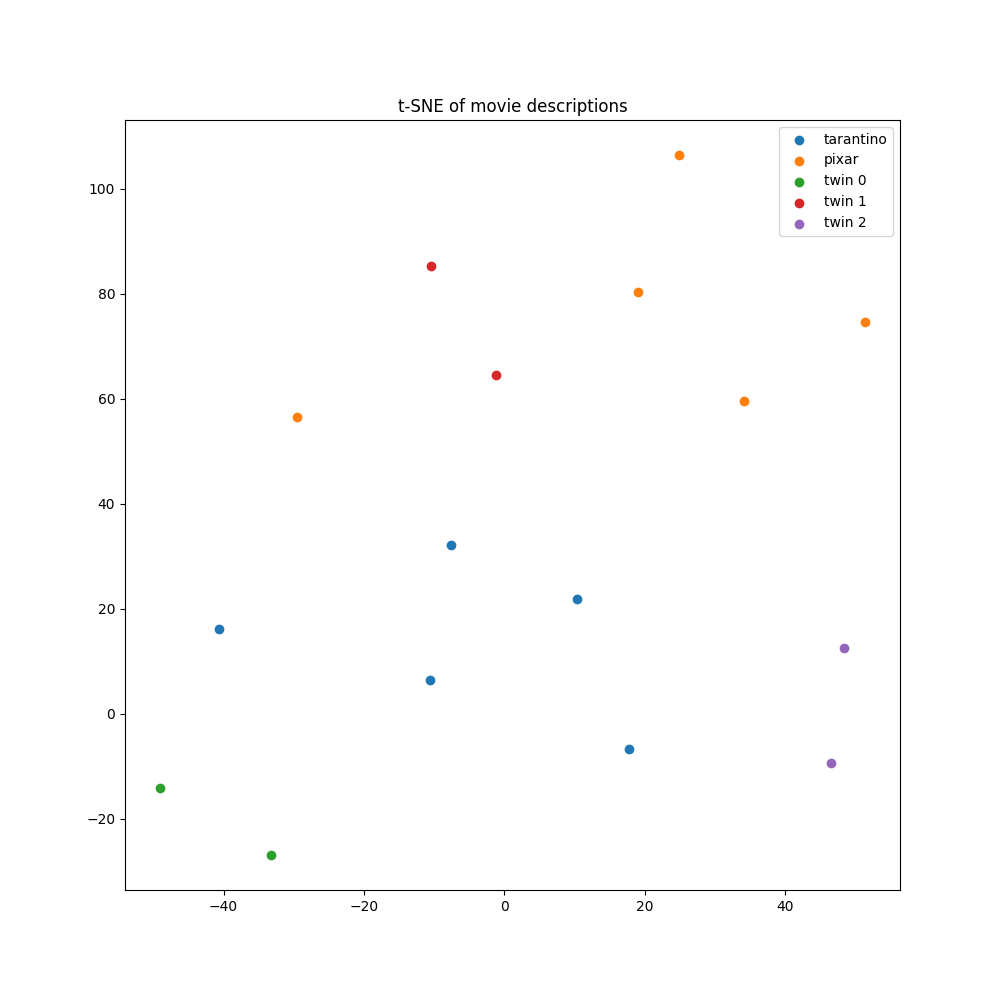
\includegraphics[width=0.8\textwidth]{tsne.png}
    \caption{t-SNE of movie descriptions}
    \label{fig:tsne}
\end{figure}

The first step on my docket is simply to construct my sample. From earlier discussions with Liran, it seems worthwhile to trim my sample of movies somehow: a couple hundred movies release each year in the US, so isolating the impact of one movie may be difficult. Given the distribution of movie performance is highly skew, it may be acceptable to focus solely on a subset of movies expected to perform well. I think limiting only to, e.g., ``top 50'' performing movies creates endogeneity concerns, as movies definitionally are in the top 50 because they perform well. However, limiting only to a handful of studios, or only to movies with a certain budget or scale of initial release (two factors set ex-ante), may be more defensible while still providing a large enough sample to work with. Per our discussion in class, this is a very clear ``doing'' task.

As far as ``thinking'' tasks go, to me the primary challenge of this paper is thinking about how to translate the text embeddings to some measure of similarity and competition. Some initial desiderata:
\begin{itemize}
    \item A movie in a more crowded market should experience more competition
    \item A movie with more similar competitors should experience more competition
\end{itemize}

How to balance these is non-obvious: how should I think about, for example, a pair of twin films in duopoly versus a distinctive film in a crowded market? 

Similarly, I need to think about how to compute distance between movies. OpenAI provides very high-dimensional embeddings, such that traditional Euclidean distance measures are not feasible under the curse of dimensionality. Some initial ideas:
\begin{itemize}
    \item The simplest (and I think weakest) answer is feeding each embedding value into a simple regression. This is a \emph{very} wide dataset, such that each component likely won't have much power. One low-cost, high-return improvement would be to apply some sort of regularization such as LASSO to trim out the less important components, identifying only the components carrying the most information. 
    \item My understanding of the literature in this space is that generally distance in text embeddings is understood via cosine similarity, representing the angle between the two embedding vectors. This works well for \emph{pairwise} distances, but is not particularly interpretable, and loses any sort of ``directionality'' in the difference.
    \item I could try to reduce the dimensionality of the embeddings. Usually in this kind of model, my understanding is a standard approach is to perform some version of PCA on the data, plot the eigenvalues corresponding to the components, and choose the set of components prior to some inflection point to reduce the number of components. I could then use these components as standard ``Xs'' in a BLP model. 
\end{itemize}

A third-year student in the econometrics group, Amar Venugopal, recently presented some preliminary work in metrics lunch on using text embeddings as a form of treatment variable. He solicited applications for this type of technique during his talk, such that I am optimistic he would find the idea compelling. If the above sounds good to you, I've considered reaching out to him to hear his thoughts, or as a potential coauthor if he finds the project a particularly good fit. 

\end{document}